\documentclass[11pt,a4paper]{article}

\usepackage{Act}

\begin{document}
\input{\detokenize{/home/fenarius/Travail/Cours/NSIPremiere/docs/commun/Macros.tex}}
\ModeActivite
\Activites{\debase\; -- C2 : Représentation des entiers et des caractères}{\Pre}

%Nom de la première activité
\begin{Exercise}[title={Compter avec des 0 et des 1}]

C'est décidé : nous allons changer de monnaie ! Fini les euros nous comptons désormais en \textit{Bin} dont le symbole est {\bbfamily B}. De toute nouveaux billets de banque ont été émis, vous en voyez la liste ci-dessous :
\begin{center}
\begin{tabularx}{0.8\textwidth}{|Y|Y|}
\hline
\rule{0pt}{64px}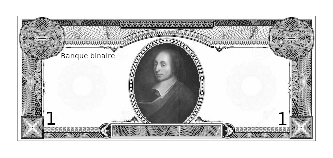
\includegraphics[scale=1]{images/pascal.eps} & 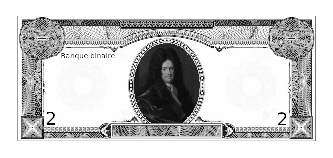
\includegraphics[scale=1]{images/leibniz.eps} \\
\hline
\rule{0pt}{64px}\includegraphics[scale=1]{images/babbage.eps} & \includegraphics[scale=1]{images/lovelace.eps} \\
\hline
\rule{0pt}{64px}\includegraphics[scale=1]{images/boole.eps} & \includegraphics[scale=1]{images/turing.eps} \\
\hline
\rule{0pt}{64px}\includegraphics[scale=1]{images/vonneumann.eps} & \includegraphics[scale=1]{images/hooper.eps}  \\
\hline
\end{tabularx}
\end{center}
\Question On suppose qu'on ne dispose que d'\textbf{un} seul exemplaire de chaque billet.
   \subQuestion Peut-on réunir exactement le somme de 73 {\bbfamily B}  ? Comment ?
    \subQuestion Même question pour 155 {\bbfamily B}.
  	\subQuestion Même question pour 218 {\bbfamily B}.
 \Question Pour simplifier l'écriture d'une somme contenant au maximum un seul de ces billets, on propose d'utiliser le tableau suivant. Dans la colonne du billet on indique \textbf{1} si le billet est utilisé et \textbf{0} sinon. Recopier et compléter le tableau ci-dessous.
 \begin{center}
\renewcommand{\arraystretch}{1.3}
 \begin{tabularx}{0.8\textwidth}{Xp{1cm}|p{1cm}|p{1cm}|p{1cm}|p{1cm}|p{1cm}|p{1cm}|p{1cm}|}
  & \multicolumn{1}{c}{\framebox{128 {\bbfamily B}}}& \multicolumn{1}{c}{\framebox{\ 64 {\bbfamily B}}} &  \multicolumn{1}{c}{\framebox{\ 32 {\bbfamily B}}} & \multicolumn{1}{c}{\framebox{\ 16 {\bbfamily B}}} & \multicolumn{1}{c}{\framebox{\ \ 8 {\bbfamily B}}} & \multicolumn{1}{c}{\framebox{\ \ 4 {\bbfamily B}}} & \multicolumn{1}{c}{\framebox{\ \ 2 {\bbfamily B}}} & \multicolumn{1}{c}{\framebox{\ \ 1 {\bbfamily B}}} \\
\hline
\multicolumn{1}{|c|}{148} & \dots &\dots &\dots &\dots &\dots &\dots &\dots &\dots  \\
\hline
\multicolumn{1}{|c|}{42} & \dots &\dots &\dots &\dots &\dots &\dots &\dots &\dots  \\
\hline
\multicolumn{1}{|c|}{237} & \dots &\dots &\dots &\dots &\dots &\dots &\dots &\dots  \\
\hline
\multicolumn{1}{|c|}{219} & \dots &\dots &\dots &\dots &\dots &\dots &\dots &\dots  \\
\hline
\multicolumn{1}{|c|}{\dots} & 0 & 0 & 0  & 0 & 0 &1 &1 &1  \\
\hline
\multicolumn{1}{|c|}{\dots} & 1 & 0 & 1  & 0 & 0 &1 &0 &0  \\
\hline
\multicolumn{1}{|c|}{\dots} & 0 & 1 & 1  & 1 & 0 &0 &0 &1 \\
\hline
\multicolumn{1}{|c|}{\dots} & 1 & 0 & 1  & 1 & 0 &1 &0 &0 \\
 \hline
  \end{tabularx}
\end{center}
    	\subQuestion Quelle somme maximale peut-on réunir en utilisant au maximum un seul de ces billets ? 
      \subQuestion Peut-on réunir n'importe quelle somme (jusqu'à la somme maximale) ? Expliquer.
      \subQuestion Les valeurs de ces billets n'ont pas été choisies au hasard, à votre avis quel doit être le montant du billet suivant ? Pourquoi ?
      \subQuestion Dans le tableau ci-dessus, que peut-on dire des nombres pour lesquels le billet 1 {\bbfamily B} n'est pas utilisé ?
      \subQuestion Proposer une méthode pour trouver les billets à utiliser pour une somme donnée.
  \Question \textbf{Question subsidiaire} : trouver les noms des personnages célèbres de l'histoire de l'informatique placés sur ces billets de banque.
\end{Exercise}
\end{document}